% 2. Fragen zur Vorbereitung

\chapter{Theoretischer Hintergrund}
\label{chap:theo}
Bevor wir uns zur Versuchsdurchführung und der Auswertung zuwenden wollen wir die Theorie von FRET näher besprechen. Dafür verwenden wir \citep{Anleitung} und \citep{Fluorescence} als Hauptquelle.

\section{FRET-Effekt}
\label{sec:dipolToFRET}
Um den FRET-Effekt zu beobachten, werden zwei Farbstoffe benötigt mit unterschiedlichen Absorptions- und Emissionsspektrum. Dabei muss sich das Emissionsspektrum des \textbf{\textit{Donor}}-Farbstoffs und das Absorptionsspektrum des \textbf{\textit{Akzeptor}}-Farbstoffs eine deutliche Überlappung aufzeigen (hellblauer Bereich in Abb. \ref{image:lappung}).\\

Durch Anregung des Donors wird das Molekül von einem Grundzustand $S_0$ in den ersten angeregten Zustand $S_1$ gebracht. Anzumerken ist aber, dass Moleküle anders, wie bei einzelnen Atomen, mehrere Energiezustände haben, darunter fällt die Energie des elektronischen Übergangs, der Schwingung und der Rotation (Gesamtenergie $E=E_{rot}+E_{vib}+E_{el}$). Das Vorhandensein von mehreren Energiezuständen hat zur Folge, dass sich Unterniveaus bilden in Fall von Molekülen entsteht ein \textit{Bandspektrum}.
\begin{center}
    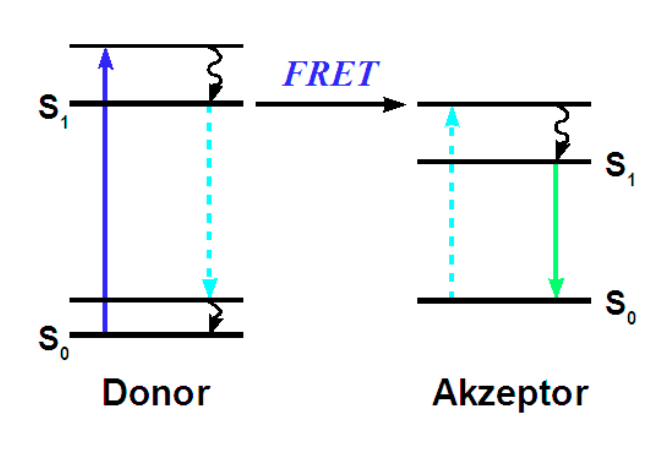
\includegraphics[scale=0.23]{FRET-Effekt.png}
    \captionof{figure}{FRET-Übergang \citep{Anleitung}}
    \label{image:FRET}
\end{center}
Durch Anregung eines Photons entsteht ein Übergang in das höhere Energieniveau $S_1$. Dieses koppelt sich an Vibrationen und verliert dabei ein Teil der Anregungsenergie des Photons. Nach der sogenannten Lebensdauer $\tau$ emittiert das Molekül spontan ein Fluoreszenzphoton und fällt in den Grundzustand $S_0$ zurück. Bei diesem Vorgang kommt es dann zur sogenannten \textit{Stokes-Verschiebung}, wodurch aufgrund des Energieverlusts die Wellenlänge des Fluoreszenzphotons höher ist als die des Anregungsphotons. Liegt nun die Wellenlänge des Fluoreszenzphotons im Absorptionsspektrum des Akzeptors geht die Anregungsenergie des Donors \textbf{\textit{strahlungslos}} auf den Akzeptor über, welcher wiederum durch Kopplung an Vibrationen ein Fluoreszenzphoton emittiert und in seinen Grundzustand zurückfällt. Diesen Vorgang nennt man \textbf{\textit{FRET-Effekt}} (siehe Abb. \ref{image:FRET}).
\newpage
\subsection*{Dipol-Dipol-Wechselwirkung und Fermis' goldene Regel}
Damit der Übergang der Energie strahlungslos vonstattengeht, muss es zu einer Dipol-Dipol.Wechselwirkung zwischen Donor und Akzeptor kommen. Dabei hängt die Effizienz des Energieübertrags von der Spektrenüberlappung, der Orientierung der Dipole und der Distanz der Farbstoffe verursacht vom Dipolfeld ab. Die Übergangswahrscheinlichkeit und die Effizienz des FRET-Effekts kann durch Fermis' goldene Regel angegeben werden:
\begin{gather}
    \abs{\left\langle \phi_{D}^* \phi_A \bigg \vert \frac{\kappa}{4\pi\epsilon_0} \frac{\mu_D\mu_A}{r^3} \bigg \vert \phi_D \phi_A^* \right\rangle }^2
\end{gather}
Dabei entspricht $\kappa$ dem winkelabhängigen Orientierungsfaktor der Dipole, $\epsilon_0$ der elektrischen Feldkonstante, $\mu_D$ dem elektrischen Dipolmoment des Donors und $\mu_A$ dem elektrischen Dipolmoment des Akzeptors. Die Abhängigkeit von $\frac{1}{r^3}$ kommt dabei von der Multipolentwicklung des Dipol-Moments und durch das quadrieren von Fermis' goldener Regel entsteht entsteht die $\frac{1}{r^6}$-Abhängigkeit in Gleichung \ref{eq:effizienz}. Die Effizienz des FRET-Effekts lässt sich dann wie folgt angeben:
\begin{gather}
    E = \frac{\text{Zahl der Energitransfers}}{\text{Zahl der Anregungen}} = \frac{k_{ET}}{k_F + k_{ET} + k_0} = \frac{R_F^6}{R_F^6+R^6}
    \label{eq:effizienz}
\end{gather}
Hierbei entspricht $R_F$ dem Försterradius und $R$ den Abstand zwischen den beiden Proben und $k_{ET}, k_F$ und $k_0$ den Raten der Energietransfers. Wenn der Abstand $R$ dem Försterradius $R_F$ entspricht, erhält man:
\begin{gather}
    E = \frac{R_F^6}{R_F^6+R^6} \overset{R = R_F}{=} \frac{1}{2}
\end{gather} 
Somit ist der Försterradius der Abstand zwischen den Proben, der einer Effizienz von 50\% entspricht.\\
Damit der FRET-Effekt auftritt sollte der Abstand $R$ zwischen Donor und Akzeptor ungefähr den Försterradius $R_F$ entsprechen. In unserem Versuch verwenden wir CFP und YFP Proben bei denen liegt der Försterradius bei einem Abstand von $R = \SI{4.9}{\nano\metre} = R_F$ \citep{Radius}. 
\subsection*{Abhängigkeit der Orientierung}
Besitzen der Donor und der Akzeptor eine feste Orientierung, verringern sich die Anzahl der Freiheitsgrade auf einen Freiheitsgrad, den Abstand. Womit die Effizienz nur vom Abstand $R$ abhängt.
\subsection*{Grenzfälle}
Beim Energietransfer sind mehrere Grenzfälle zu beachten, darunter fallen einen parallele oder eine orthogonale Orientierung der Moleküle zueinander. Bei paralleler Ausrichtung ist der Energietransfer am besten, während bei orthogonaler Ausrichtung keine Energie übertragen wird.
\subsection*{FRET-Effekt umgekehrt möglich?}
\begin{center}
    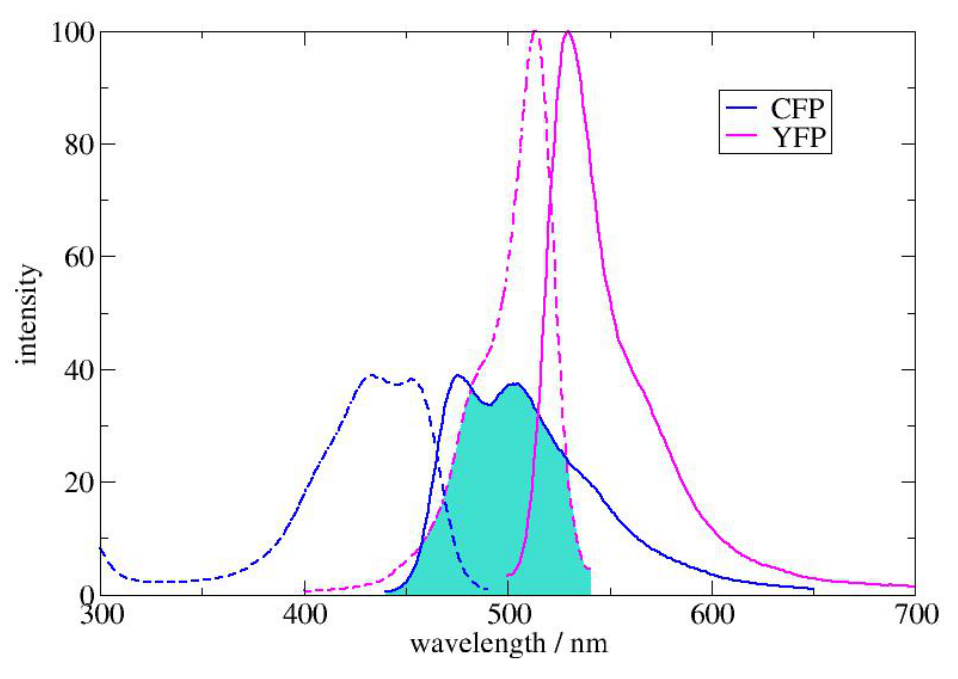
\includegraphics[scale=0.2]{Ueberlappung.png}
    \captionof{figure}{Anregungs- und Emissionsspektrum von CFP und YFP \citep{Anleitung}}
    \label{image:lappung}
\end{center}
Die Vorraussetzung für FRET ist die Überlappung des Emissionsspektrums des Donors und des Absorptionsspektrums des Akzeptors. Diese Vorraussetzung ist bei CFP als Donor und YFP als Akzeptor erfüllt (Durchgezogene blaue Linie zeigt deutliche Überlappung mit gestrichelter pinken Linie in Abb. \ref{image:lappung}). Vertauscht man aber die Rollen von CFP und YFP ist keinen Überlappung mehr gegeben (Durchgezogene pinke Linie schneidet gestrichelte blaue Linie nicht in Abb. \ref{image:lappung} und somit keine Überlappung). Damit ist in diesem Versuch keine FRET-Effekt mit YFP möglich.
\section{Crosstalk-Verunreinigungen}
\label{sec:verunreinigung}
\begin{center}
    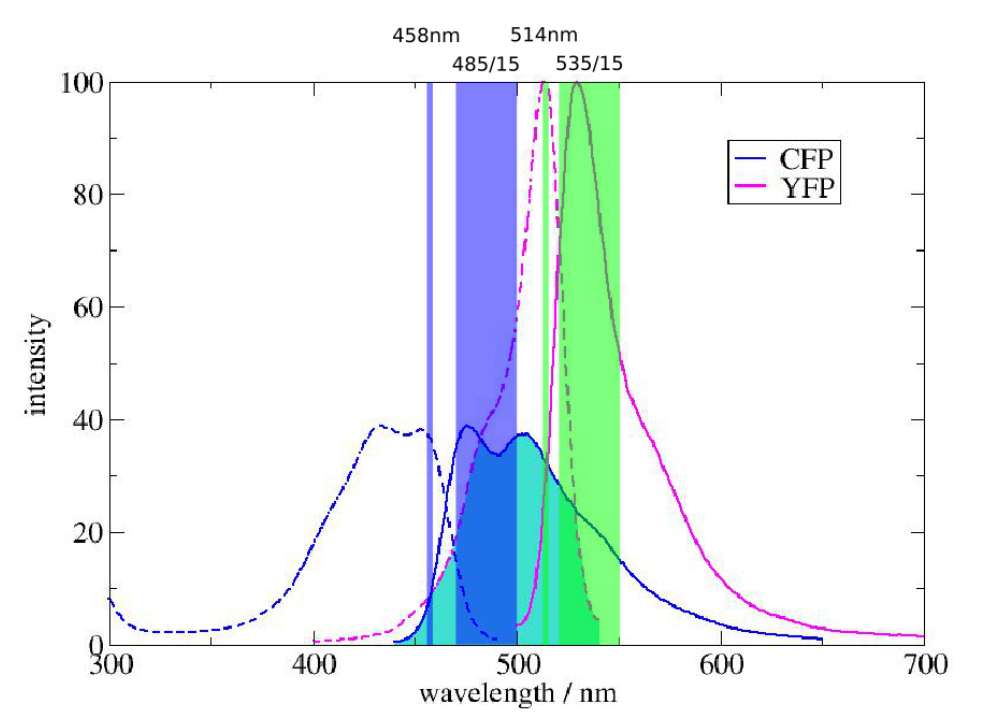
\includegraphics[scale=0.2]{Anregungslinien.png}
    \captionof{figure}{Anregungsbereiche von CFP und YFP \citep{Anleitung}}
    \label{image:anregung}
\end{center}
Die FRET-Intensität kann man nicht direkt messen, da sich der Anregungsbereich der Donors und Akzeptors teilweise überlappen (siehe Abb. \ref{image:anregung}). Somit wird bei einer Anregung des Donors auch der Akzeptor angeregt. Dies führt zu Verunreinigungen in der Messung der Emission des Akzeptors durch die teilweise Anregung. Um diesen Effekt zu korrigieren, misst man die Emission des Donors und die Emission des Akzeptors separat, womit man die Crosstalk Beiträge berechnen kann.
\section{Zeitkorrelierte Einzelphotonenzählung}
Allgemein ist zeitkorrelierte Einzelphotonenzählung (englisch time-correlated single photon counting, TCSPC) eine Technik, um sich zeitlich schnell ändernden Lichtintensitäten zu messen. Diese Messmethode kommt zum Einsatz bei der Messung von Fluoreszenzlebenszeit. Dabei wird die zu untersuchende Probe (Fluorophore) mithilfe von gepulsten Lichtbündel (Laser) angeregt. Die Detektion der Fluoreszenz erfolgt mit einem Photomultiplier, welcher einzelne Photonen registrieren können muss. Die Zeitmessung wird dann durch die Anregung des Laserpuls gestartet und das emittierte Photon stoppt diese. Die Messung wird wiederholt und die einzelnen Photonen werden, mit ihrer entsprechenden Zeit, in ein Histogramm eingetragen. Dieses zeigt einen exponentiellen Abfall der Fluoreszenzintensität nach der Anregung. Der Abfall ergibt sich dann mit der Formel:
\begin{gather}
    N(t) = N_0e^{-\frac{t}{\tau}}~\text{mit}~\frac{1}{\tau} = \sum^m_{i=1} k_i \xrightarrow{n~\text{Proben}} N(t) = \sum_{i=1}^n N_ie^{-\frac{t}{\tau_i}} 
\end{gather} 
Hierbei ist $\tau$ die Lebenszeit aus den $m$ einzelnen Zerfallsraten $k_i$ und $\tau_i$ die Lebenszeit der i-ten Probe mit entsprechender Amplitude $N_i$.\\
Das detektiert Signal hat dann die Form einer Faltung von dem exponentiellen Abfall und einer Gauß-Kurve (entsteht durch die IRF (Impulse Response Function) des Lasers), welches in Abb. \ref{image:abfall} zu sehen ist. Dabei ist der Teil bis zum Peak die IRF und danach der exponentielle Abfall.
\begin{center}
    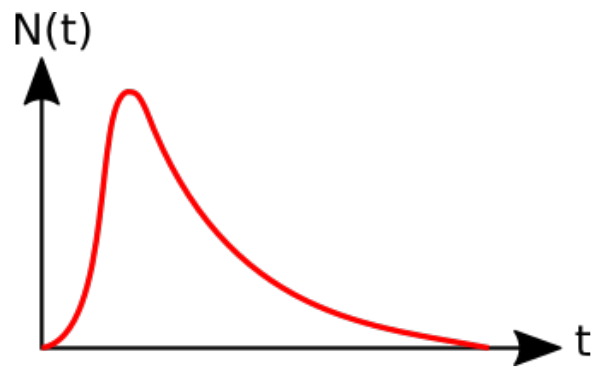
\includegraphics[scale = 0.3]{Abfall.png}
    \captionof{figure}{Verlauf der zeitkorrelierten Einzelphotonenzählung \citep{Anleitung}}
    \label{image:abfall}
\end{center}
\newpage
\subsection*{Störungen}
Bei dieser Messtechnik kann es allerdings zu Störungen kommen, welche das Ergbnis verfälschen.Dazu gehört das thermische Rauschen, wovon beinahe jedes Messgerät betroffen ist. Dies kann durch Kühlung des Messgerätes behoben werden.\\Weitere Störungsfaktoren, sogenannte ’Dark Counting’, sind \textit{Verstärkerrauschen}, \textit{'Afterpulsing'} und \textit{Pile-Up Effekt}.
\begin{itemize}
    \item[(1)] Das \textit{Verstärkerraschen} entsteht durch den angeschlossenen Photomultiplier und lässt sich mit einem Hochpassfilter lösen, da die Amplituden des Rauschens meist geringer sind als die Amplituden der eigentlichen Messung.
    \item[(2)] Beim \textit{'Afterpulsing'} registriert der Detektor nach dem Photonenereignis eine weiteres (fiktives) Ereignis. Behoben kann dies mit der richtigen Wahl des Detektors.
    \item[(3)] Der \textit{Pile-Up Effekt} entsteht durch den Umstand, dass eigentlich nur ein Photon pro Laserpuls mit der Probe wechselwirken kann. Bei mehreren Photonen registriert der Detektor nur das erste Photon, wodurch sich die gemessene Lebensdauer des Photons verringert. Verantwortlich für diesen Effekt ist die Totzeit des Detektors. In dieser Totzeit kann der Detektor kein weiteres Photon detektieren. Verringerung der Laserintensität kann dem Effekt entgegenwirken. \citep{Time}
\end{itemize} 
\newpage
\section{In diesem Versuch verwendete Proben}
\label{sec:proben}
Die verwendeten Proben in diesem Versuch werden mit einem Farbstoff markiert (Proben gehen kovalente Bindung mit Farbstoff-Molekül ein). Bei Anregung emittiert die Probe sichtbare Probe, was den Sachverhalt der Fluoreszenz darstellt.
\begin{center}
    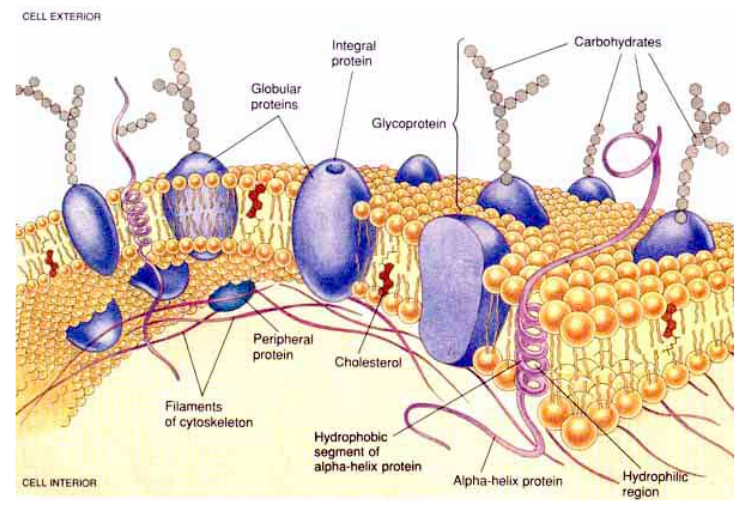
\includegraphics[scale=0.35]{Membran.png}
    \captionof{figure}{Skizze des Plasmamembran \citep{Anleitung}}
    \label{image:membran}
\end{center}
Die genutzte Zelle besitzen ein Plasmamembran, welches aus verschiedenen Lipiden aufgebaut ist (siehe Abb. \ref{image:membran}). Unterhalb der Lipiden sind ca. 30\% Phospholipide und Phosphatidylinositol(4,5)-Bisphosphat (PIP2). PIP2 ist besonders, denn es binden sich im Zellplasma vorhandenen Pleckstrin-Homologiedomäne (PH). In unserem Versuch wird dies verwendet, um CFP und YFP an Proteine mit einer solchen Pleckstrin-Homologiedomäne zu bindet. Durch die hohe Dichte an PIP2 binden sich viele CFP-PH und YFP-PH an das PIP2. Dies hat zur Folge, dass die Distanz zwischen YFP (Akzeptor) und CFP (Donor) gering genug ist, damit die Bedingung für FRET erfüllt ist.
\section{Photobleaching}
\label{sec:bleaching}
Das Photobleaching (dt. Bleichen) ist ein irreversibler Mechanismus, bei dem es zu einem Verlust der Fluoreszenzvon Fluorophoren kommt. Beim Bleaching wird das Fluorophor mit Licht bestrahlt, womit Photonen mit unterschiedlichen Energien auf die Probe treffen. Diese Photonen können vom Fluorophor absorbiert werden und es zu einem Übergang in einen angeregten Zustand (siehe Kapitel \ref{sec:dipolToFRET}). Durch Wechselwirkung zwischen dem angeregten Fluorophor und der Umgebung, kommt es zu einer kovalenten Änderung des Fluorophors, wodurch das Fluorophor seine Fluoreszenz verliert\\ Weiterhin kann man das Fluorophor mithilfe von Quenching (dt. Fluoreszenzlöschung) bleichen, dabei kommt es zu einer Abnahme der Fluoreszenz. Dieser Prozess ist aber zum Gegensatz zum Photobleaching reversibel. \citep{Bleach}
\section{Konfokalmikroskop}
\label{sec:konfokal}
Ein Konfokalmikroskop ist ein spezielles Lichtmikroskop, welches zu jedem Zeitpunkt nur einen Teil der Probe beleuchtet und genau dieser Bruchteil wird dann Stück für Stück abgerastert.
\subsection*{Funtionsweise}
\begin{center}
    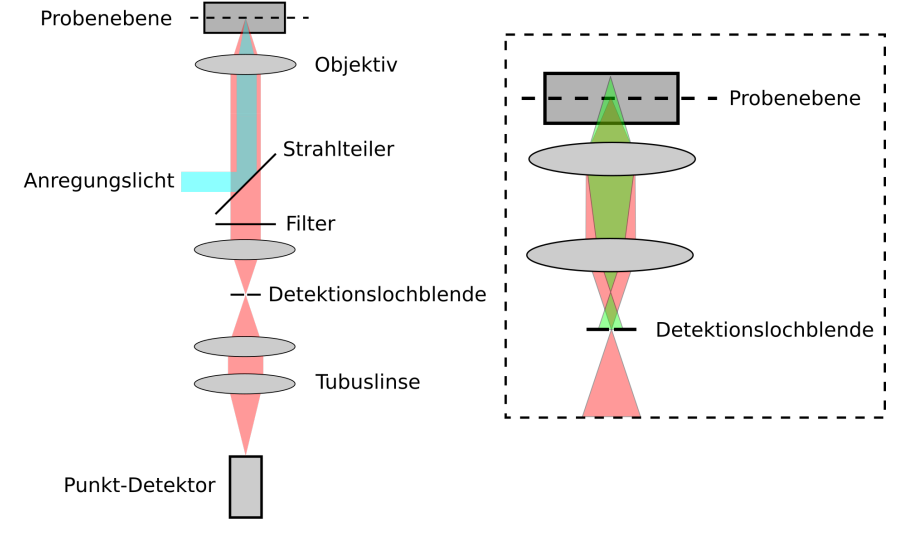
\includegraphics[scale=0.27]{Konfokallinsen.png}
    \captionof{figure}{Prinzipieller Aufbau eines Konfokalmikroskop \citep{Anleitung}}
    \label{image:konfokal}
\end{center}
In Abb. \ref{image:konfokal} wird der prinzipielle Aufbau eines Konfokalmikroskop gezeigt. Dabei wird der Anregungsstrahl (blau in \ref{image:konfokal}) durch einen Strahlenteiler reflektiert und durch eine Linse gebündelt mit dem Brennpunkt auf der Probe. Von der Probe wird dann der sogenannte Detektionsstrahl (rot in \ref{image:konfokal}) ausgesendet. Dieser Strahl wird durch die oberste Linse parallelisiert und trifft auf den Strahlenteiler, der den Strahl transmittieren lässt. Nach dem Strahlenteiler kann ein Filter eingebaut werden, welcher die störenden Wellenlängen herausfiltert. Nach dem Filter befindet sich eine weitere Linse und die Detektionslochblende, welche das Detektionsvolumen auf einen kleinen Bereich einschränkt. Dies bedeutet das Strahlen aus einem hinteren Bereich der Probe nicht zum Detektor gelangen. Nach der Blende trifft der Detektionsstrahl auf die erste Tubuslinse. Diese parallelisiert den Strahl erneut und die zweite Tubuslinse fokussiert ihn auf den Punkt-Detektor. Der Punkt-Detektor registriert dann die einzelnen Photonen.
\subsection*{Vor und Nachteile}
\begin{itemize}
    \item[\textcolor{green}{\textbf{+}}] Unerwünschtes Hintergrundrauschen (z.B. Streulicht) reduzierbar auf ein Minimum und bessere Auflösung zum Vergleich zu konventionellen Mikroskopen wegen der Detektionslochblende
    \item[\textcolor{red}{\textbf{-}}] Detektionslochblende kann Beugungserscheinungen verursachen, was die Auflösung begrenzt
\end{itemize}
Als Alternative zum Konfokalmikroskop kann das Laser-Scanning-Microscope verwendet werden, welches ohne die Detektionslochblende auskommt und eine höhere Auflösung besitzt.